\documentclass[11pt]{article}
\usepackage[utf8]{inputenc}
\usepackage[russian]{babel}
\usepackage[T1]{fontenc}
\usepackage{amssymb,amsmath,clrscode,graphicx,indentfirst}

\author{Олег Смирнов}
\title{Курс kiev-clrs -- Лекция 2. Асимптотическая нотация}
\date{21 марта 2009 г.}

\begin{document}
\maketitle
\tableofcontents

\newpage
\setlength{\parskip}{1ex plus 0.5ex minus 0.2ex}
\section{Цель лекции}
\begin{itemize}
\item Ввести строгие математические определения для $O$-, $\Omega$- и $\Theta$-нотации 
\item Рассмотреть методы решения рекурентностей: подстановка, дерево рекурсии и основной метод
\end{itemize}

\section{Асимптотическая нотация}

\subsection{$O$-обозначения}
В случае, когда необходимо определить только \emph{асимптотическую верхнюю границу}, используют $O$-обозначения:
\begin{equation*}
  f(n) = O(g(n)) \Rightarrow \exists c, n_0 > 0 \text{ такие, что }
  0 \leqslant f(n) \leqslant c g(n), \forall n > n_0
\end{equation*}

$O(g(n))$ можно рассматривать как множество функций:
\begin{equation*}
  O(g(n)) = \{f(n): \exists c, n_0 > 0 \text{ такие, что }
  0 \leqslant f(n) \leqslant c g(n), \forall n > n_0
  \}
\end{equation*}

Пример:
\begin{equation*}
  2n^3 = O(n^3) \text{ для } c = 1, n_0 = 2 \text{ или } 2n^3 \in O(n^3)
\end{equation*}

Определение через множество можно использовать в качестве ``макроса''
-- $O$-нотация в формуле обозначает некоторую функцию из соответствующего семейства.

Пример:
\begin{equation*}
  n^2 + O(n) = O(n^2) \text{ означает } \forall f(n) \in O(n): \exists h(n) \in O(n^2): n^2 + f(n) = h(n)
\end{equation*}

\subsection{$\Omega$-обозначения}

Для определения \emph{асимптотическую нижней границы} есть $\Omega$-обозначение:
\begin{equation*}
  \Omega(g(n)) = \{f(n): \exists c, n_0 > 0 \text{ такие, что }
  0 \leqslant c g(n) \leqslant f(n), \forall n > n_0
  \}
\end{equation*}

Пример:
\begin{equation*}
  \sqrt(n) = \Omega(\lg n) \text{ для } c = 1, n_0 = 16
\end{equation*}

\subsection{$\Theta$-обозначения}

Для точной оценки используется $\Theta$-обозначение. Его можно ввести несколькими способами:
\begin{itemize}
\item Теорема: для любых двух функций $f(n)$ и $g(n)$ соотношение $f(n)~=~\Theta(g(n))$ верно тогда и только тогда, когда $f(n)~=~O(g(n))$ и $f(n)~=~\Omega(g(n))$
\item Пересечение множеств: $f(n)~=~\Theta(g(n))$ $\iff$ $f(n)~=~O(g(n))~\cap~\Omega(g(n))$
\end{itemize}

Пример:
\begin{equation*}
  \frac{1}{2}n^2 - 2n = \Theta(n^2)
\end{equation*}

\subsection{$o$- и $\omega$-обозначения}

$o$- и $\omega$-обозначения являются версиями определений $O$ и $\Omega$, которые выполняются 
\emph{для любой константы $c$}, т.е. не являются асимптотически строгими. Формально:
\begin{equation*}
  o(g(n)) = \{f(n): \forall c > 0: \exists n_0 > 0 \text{ такое, что }
  0 \leqslant f(n) \leqslant c g(n), \forall n > n_0
  \}
\end{equation*}
Функция $f(n)$ пренебрежима мала по сравнению с функцией $g(n)$ при $n$ стремящемся к бесконечности, т.е.: 
\begin{equation*}
  \lim_{n\to\infty}\frac{f(n)}{g(n)} = 0
\end{equation*}
Пример:
\begin{equation*}
  2n^2 = o(n^3) \text{ для } n_0 = \frac{2}{c}
\end{equation*}
Аналогично:
\begin{equation*}
  \omega(g(n)) = \{f(n): \forall c > 0: \exists n_0 > 0 \text{ такое, что }
  0 \leqslant c g(n) \leqslant f(n), \forall n > n_0
  \}
\end{equation*}
Пример:
\begin{equation*}
  \sqrt(n) = \omega(\lg n) \text{ для } n_0 = 1 + \frac{1}{c}
\end{equation*}

\subsection{Некоторые свойства}

Из определений вытекают некоторые свойства асимтотических сравнений:

\begin{itemize}
\item Транзитивность
\begin{align*}
  f(n) = \Theta(g(n)) \land g(n) = \Theta(h(n)) \Rightarrow f(n) = \Theta(h(n)) \\
  f(n) = O(g(n)) \land g(n) = O(h(n)) \Rightarrow f(n) = O(h(n)) \\
  f(n) = \Omega(g(n)) \land g(n) = \Omega(h(n)) \Rightarrow f(n) = \Omega(h(n)) \\
  f(n) = o(g(n)) \land g(n) = o(h(n)) \Rightarrow f(n) = o(h(n)) \\
  f(n) = \omega(g(n)) \land g(n) = \omega(h(n)) \Rightarrow f(n) = \omega(h(n))
\end{align*}

\item Рефлексивность
\begin{align*}
  f(n) = \Theta(f(n)) \\
  f(n) = O(f(n)) \\
  f(n) = \Omega(f(n))
\end{align*}

\item Симметричность
\begin{equation*}
  f(n) = \Theta(g(n)) \iff g(n) = \Theta(f(n))
\end{equation*}

\item Перестановочная симметрия
\begin{align*}
  f(n) = O(g(n)) \iff g(n) = \Omega(f(n)) \\
  f(n) = o(g(n)) \iff g(n) = \omega(f(n))
\end{align*}
\end{itemize}

Таким образом можно провести аналогию между символами нотации и операциями
сравнения рациональных чисел:
\begin{align*}
  f(n) = \Theta(g(n)) \approx f(n) = g(n) \\
  f(n) = O(g(n)) \approx f(n) \leqslant  g(n) \\
  f(n) = \Omega(g(n)) \approx f(n) \geqslant g(n) \\
  f(n) = o(g(n)) \approx f(n) < g(n) \\
  f(n) = \omega(g(n)) \approx f(n) > g(n)
\end{align*}

\section{Рекуррентные соотношения}

По определению, рекуррентное соотношение -- это уравнение или неравенство,
описывающее функцию с использованием её самой, но только с меньшими аргументами.
Обычно рекуррентное соотношение описывается в виде системы граничных условий
и формулы для общего случая, например:

\begin{equation*}
  T(n) = \begin{cases}
    \Theta(1), \text{ если } n = 1 \\
    2\Theta(n/2) + \Theta(n), \text{ если } n > 1
    \end{cases}
\end{equation*}

Для решения таких соотношений использутся несколько методов: подстановки, деревьев
рекурсии и основной метод.

\section{Метод подстановки}

Метод состоит из трех шагов:
\begin{itemize}
\item делается догадка о виде решения
\item с помощью метода математической индукции доказывается, что решение правильное
\item вычисляются константы 
\end{itemize}

\subsection{Примеры решения}
\begin{equation*}
	T(n) = 4T(n/2) + n
\end{equation*}
\begin{itemize}
\item случаи $O$ и для $\Omega$ рассматриваются отдельно
\item догадка: $T(n) = O(n^3)$
\item пусть $T(k) \leqslant c k^3$ для $k < n$ (гипотеза)
\item необходимо доказать методом мат. индукции, что $T(n) \leqslant c n^3$
\end{itemize}
\begin{align*}
  T(n) = 4T(n/2) + n \\
    \leqslant 4c(n/2)^3 + n \\
    = (c/2)n^3 + n \\
    = c n^3 - ((c/2)n^3 -n) \\
    \leqslant c n^3
\end{align*}

Неравнство выполняется, когда ``остаточная часть'' $(c/2)n^3 -n$ больше нуля, т.е. для любой константы $c \geqslant 2$ и $n \geqslant 1$.

Доказательство базового случая:
\begin{align*}
  T(n) = \Theta(1), n < n_0 \\
    1 \leqslant n < n_0 \\
    \Theta(1) \leqslant c n^3 \\
    \text{для всех достаточно больших } c
\end{align*}

Доказательство строгой верхней границы:
\begin{itemize}
\item необходимо доказать: $T(n) = O(n^2)$
\item пусть $T(k) \leqslant c k^2$ для $k < n$ (гипотеза)
\end{itemize}
\begin{align*}
  T(n) = 4T(n/2) + n \\
    \leqslant 4c(n/2)^2 + n \\
    = c n^2 + n \\
    = O(n^2)
\end{align*}
-- неверно, т.к. необходимо доказать индукционную гипотезу
\begin{align*}
    = c n^2 - (-n)\\
    \leqslant c n^2
\end{align*}
-- неверно для всех $c > 0$

Необходимо усилить индукционную гипотезу через вычитание члена более низкого порядка:
\begin{itemize}
\item пусть $T(k) \leqslant c_1 k^2 - c_2 k$ для $k < n$
\end{itemize}
\begin{align*}
  T(n) = 4T(n/2) + n \\
    = 4(c_1(n/2)^2 - c_2(n/2)) + n \\
    = c_1 n^2 - 2c_2 n + n \\
    = c_1 n^2 - c_2 n - (c_2 n - n) \\
    \leqslant c_1 n^2 - c_2 n \\
    \text{если } c_2 \geqslant 1
\end{align*}
Верно для достаточно больших $c_1$. Строгая нижняя граница доказывается по аналогии.

\section{Метод деревьев рекурсии}
\begin{itemize}
\item изображается дерево, в узлах которого находится время, требуемое для выполнения данной позадачи
\item значение времени суммируется в пределах уровня, затем -- по всем уровням дерева
\item подходит для получения ``догадки'' о виде решения для метода подстановок
\end{itemize}

\subsection{Примеры решения}
\begin{equation*}
  T(n) = T(n/4) + T(n/2) + n^2 
\end{equation*}

Для задачи размером $n$, на каждом шаге рекурсивно решается задача размером $n/4$ и $n/2$. Нерекурсивная часть выполняется за $n^2$ итераций.

После построения дерева (см. рис. \ref{fig:rectree1} - \ref{fig:rectree6}), ответом будет сумма геометрической прогрессии $n^2(1+5/6 + (5/6)^2 + (5/6)^3 + ...) = \Theta(n^2)$

\section{Основной метод}

Основной метод применятся для решения рекуррентных соотношений вида
\begin{equation*}
T(n) = aT(n/b) + f(n)
\end{equation*}
где $a \geqslant 1$, $b > 1$ -- константы, а $f(n)$ -- асимптотически положительная функция.

Рекуррентное соотношение описывает время работы алгоритма, в котором задача размером $n$
разбивается на $a$ вспомогательных задач, размером $n/b$ каждая, где $a$ и $b$ -- положительные константы.
Полученные в результате разбиения подзадачи решаются рекурсивным методом, причем время их решения
равно $Т(a/b)$. Время, требуемое для разбиения задачи и объединения результатов, полученных при
решении вспомогательных задач, описывается функцией $f(n)$.

При использовании основного метода функция $f(n)$ сравнивается с $n^{\log_b a}$ и рассматриваются три случая. Интуитивно понятно, что асимптотическое поведение решения рекуррентного соотношения определяется большей из двух функций.

\begin{itemize}
\item Если $f(n) = O(n^{\log_{b}{a - \epsilon}})$ , для некоторой константы $\epsilon > 0$, т.е. $f(n)$ растет полиноминально медленней чем $n^{log{b}{a}}$ в $n^\epsilon$ раз.\\
Тогда $T(n) = \Theta(n^{\log_b a})$

\item Если $f(n) = \Theta(n^{\log_{b}{a}}\lg^k n)$, т.е. $f(n)$ и $n^{log{b}{a}}$ растут с одинаковой скоростью с точностью до множителя $\lg^k n$, для константы $k \geqslant 0$.\\
Тогда $T(n) = \Theta(n^{\log_b a}\lg^{k+1} n)$

\item Если $f(n) = \Omega(n^{\log_{b}{a + \epsilon}})$ , для некоторой константы $\epsilon > 0$, т.е. $f(n)$ растет полиноминально быстрей чем $n^{log{b}{a}}$ в $n^\epsilon$ раз \\
\emph{и} $f(n)$ удовлетворяет неравнеству $a f(n/b) \leqslant c f(n)$ для некоторого $c < 1$\\
Тогда $T(n) = \Theta(f(n))$
\end{itemize}

Важно понимать, что этими тремя случаями не исчерпываются все возможности поведения функции $f(n)$.
Между случаями 1 и 2 есть промежуток, в котором функция $f(n)$ меньше функции $n^{\log_b a}$,
но не полиномиально меньше. Аналогичный промежуток имеется между случаями 2 и 3, когда функция
$f(n)$ не полиномиально больше. Если функция $f(n)$ попадает в один из этих промежутков, или если
для нее не выполняется условие регулярности из случая 3, основной метод неприменим.

\subsection{Примеры решения}

\begin{equation*}
  T(n) = 4T(n/2) + n
\end{equation*}
\begin{equation*}
  a = 4, b = 2 \Rightarrow n^{\log_b a} = n^2; f(n) = n
\end{equation*}

Случай 1: $f(n) = O(n^{2 - \epsilon})$ для $\epsilon = 1$

Ответ: $T(n) = \Theta(n^2)$

\begin{equation*}
  T(n) = 4T(n/2) + n^2
\end{equation*}
\begin{equation*}
  a = 4, b = 2 \Rightarrow n^{\log_b a} = n^2; f(n) = n^2
\end{equation*}

Случай 2: $f(n) = \Theta(n^2 \lg^0 n)$

Ответ: $T(n) = \Theta(n^2 \lg n)$

\begin{equation*}
  T(n) = 4T(n/2) + n^3
\end{equation*}
\begin{equation*}
  a = 4, b = 2 \Rightarrow n^{\log_b a} = n^2; f(n) = n^3
\end{equation*}

Случай 3: $f(n) = \Omega(n^{2 + \epsilon})$, для $\epsilon = 1$ и $4(n/2)^3 \leqslant c n^3$ для $c = 1/2$

Ответ: $T(n) = \Theta(n^3)$

\begin{equation*}
  T(n) = 4T(n/2) + \frac{n^2}{\lg n}
\end{equation*}
\begin{equation*}
  a = 4, b = 2 \Rightarrow n^{\log_b a} = n^2; f(n) = \frac{n^2}{\lg n}
\end{equation*}

Основной метод неприменим, т.к. для любой константы $\epsilon > 0$ справедливо $n^{\epsilon} = \omega({\lg n})$

\pagebreak
\begin{figure}[p]
  \centering
  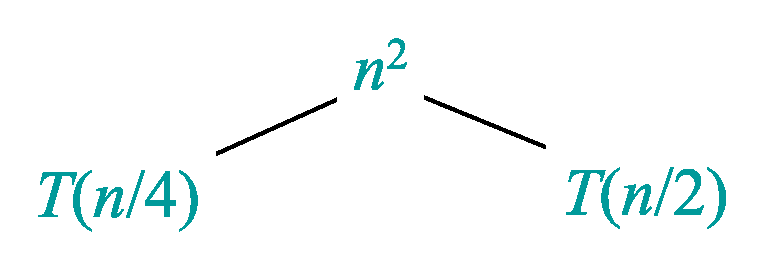
\includegraphics[width=2in]{lecture2/tree1.eps}
  \caption{Дерево рекурсии -- шаг 1}
  \label{fig:rectree1}
\end{figure}

\begin{figure}[p]
  \centering
  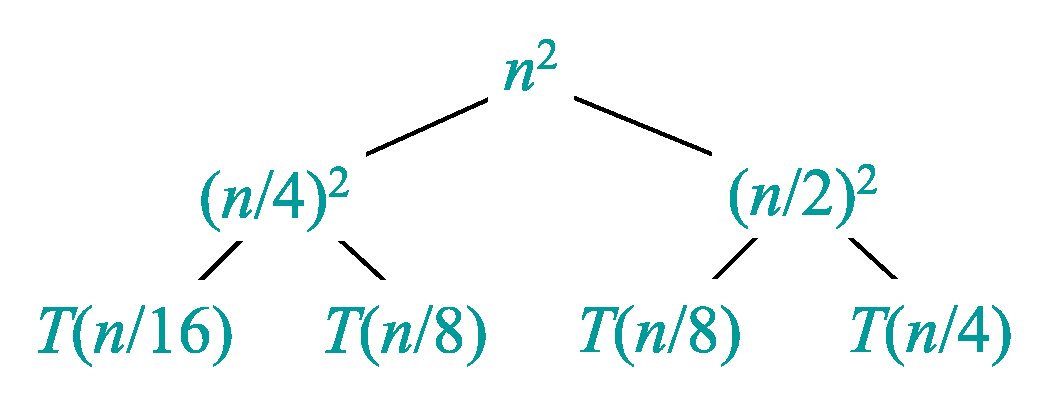
\includegraphics[width=3in]{lecture2/tree2.eps}
  \caption{Дерево рекурсии -- шаг 2}
  \label{fig:rectree2}
\end{figure}

\begin{figure}[p]
  \centering
  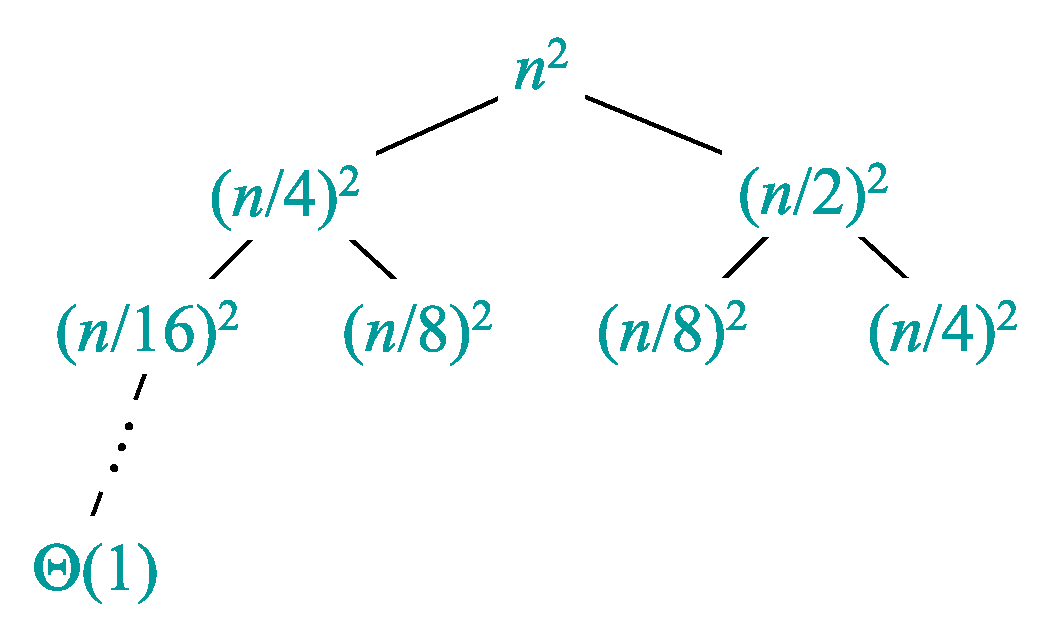
\includegraphics[width=3in]{lecture2/tree3.eps}
  \caption{Дерево рекурсии -- шаг 3}
  \label{fig:rectree3}
\end{figure}

\begin{figure}[p]
  \centering
  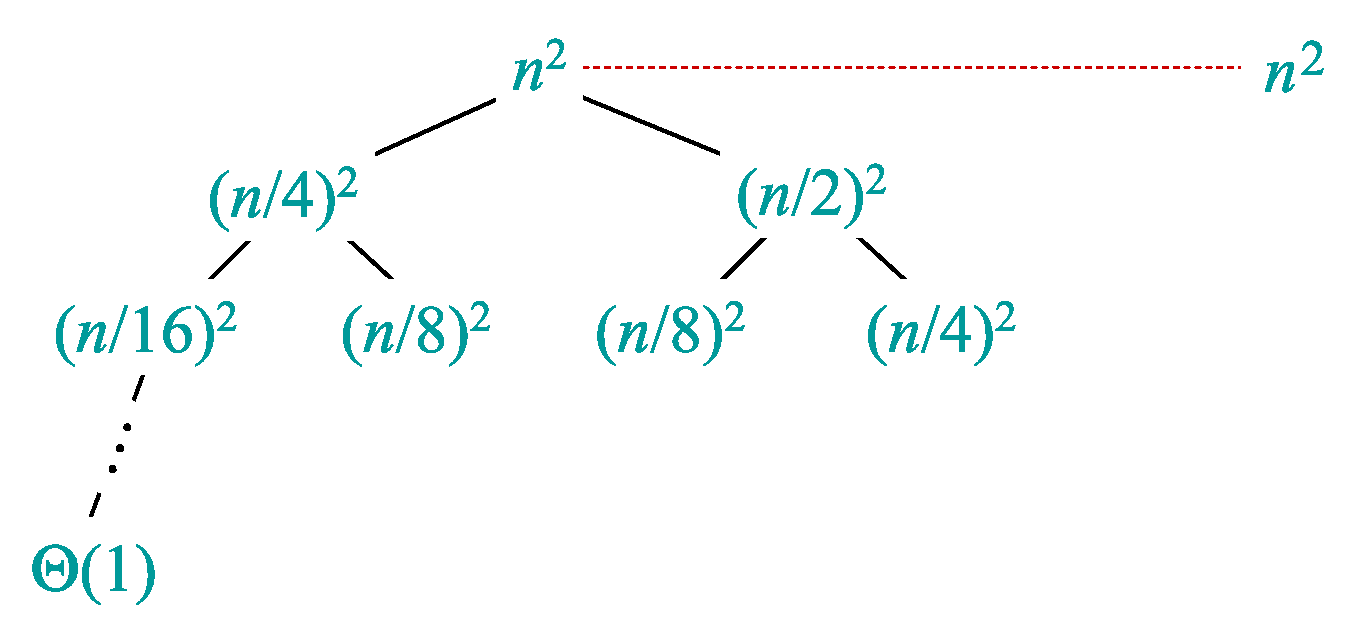
\includegraphics[width=3in]{lecture2/tree4.eps}
  \caption{Дерево рекурсии -- шаг 4}
  \label{fig:rectree4}
\end{figure}

\begin{figure}[p]
  \centering
  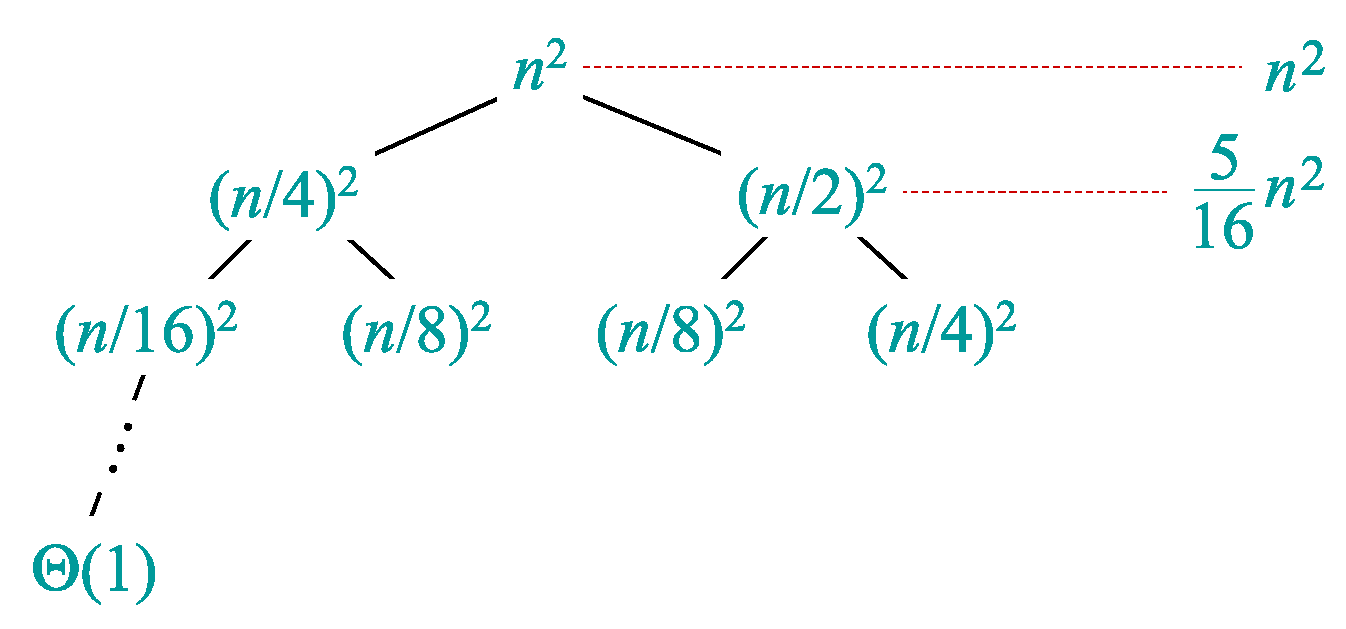
\includegraphics[width=3in]{lecture2/tree5.eps}
  \caption{Дерево рекурсии -- шаг 5}
  \label{fig:rectree5}
\end{figure}

\begin{figure}[p]
  \centering
  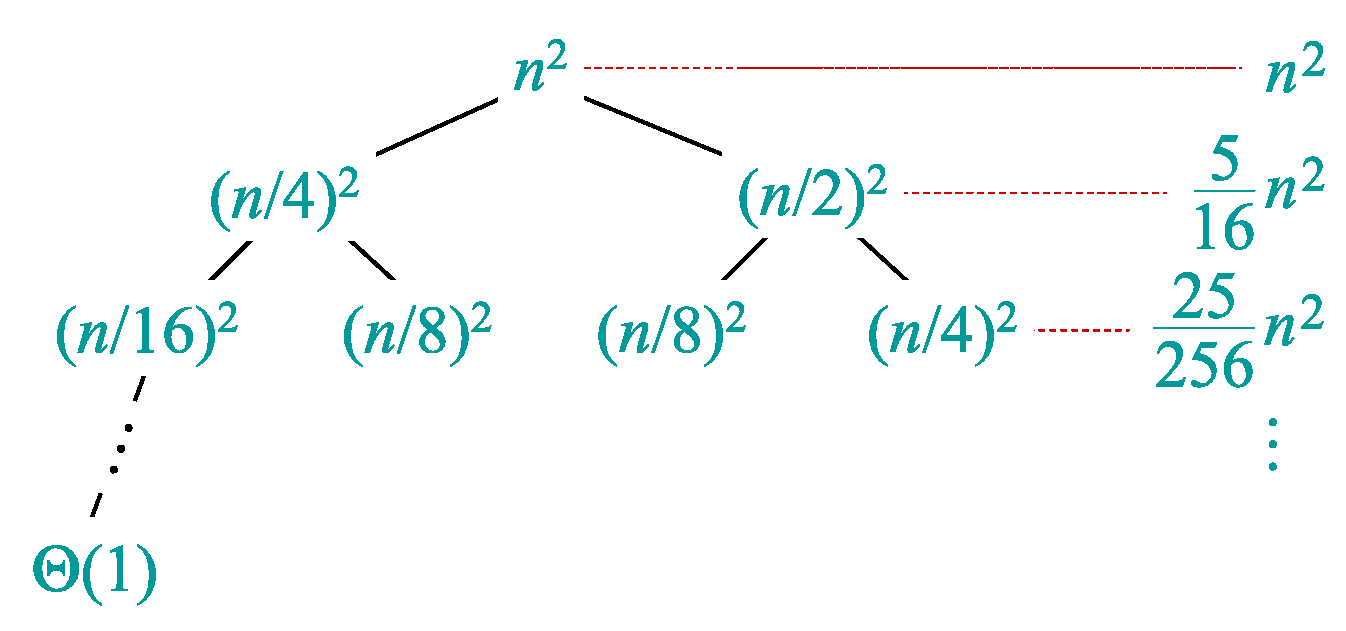
\includegraphics[width=3in]{lecture2/tree6.eps}
  \caption{Дерево рекурсии -- шаг 6}
  \label{fig:rectree6}
\end{figure}
\end{document}
